\documentclass[12pt]{article}
\usepackage[spanish]{babel}

%%%%%%%%%%%%%%%%%%%%%%%%%%%%%%%%%%
%%%%%%%%%%%%%%%%%%%%%%%%%%%%%   %%
%%        Datos Trabajo     %%  %%
%%%%%%%%%%%%%%%%%%%%%%%%%%%%%%%%%%
\newcommand{\titulo}[0]{Evidencia de aprendizaje:\\“Paradigmas de la Investigación”}
\newcommand{\materia}[0]{Fundamentos de Investigación}
\newcommand{\grupo}[0]{BI-BFIN-2002-B2-013}
\newcommand{\unidad}[0]{Unidad 1}


%%%%%%%%%%%%%%%%%%%%%%%%%%%%%%%%%%
%%%%%%%%%%%%%%%%%%%%%%%%%%%%%%%%%%
\usepackage{amssymb}
\usepackage{enumerate}
\usepackage{geometry}
\usepackage{mathtools}
\usepackage{multicol}
\usepackage{soul}

\usepackage{graphicx}
	\graphicspath{ {assets/} }

\usepackage{hyperref}
	\hypersetup{
			pdftex,
		        pdfauthor={bench},
		        pdftitle={\titulo},
		        pdfsubject={\materia},
		        pdfkeywords={\grupo, \unidad, UnADM},
		        pdfproducer={Latex with hyperref, Ubuntu},
		        pdfcreator={pdflatex, or other tool},
			colorlinks=true,
				linkcolor=red,
				urlcolor=cyan,
				filecolor=yellow,
				citecolor=blue}

%%%%%%%%%%%%%%%%%%%%%%%%%%%%%%%%%%
%%%%%%%%%%%%%%%%%%%%%%%%%%%%%%%%%%

\title{
	
\includegraphics{../../../assets/logo-unadm} \\
	\ \\ Benjam\'in Rivera \\
	\bf{\titulo}\\\ \\}

\author{
	Universidad Abierta y a Distancia de México \\
	TSU en Biotecnolog\'ia \\
	\textit{Materia:} \materia \\
	\textit{Grupo:} \grupo \\
	\textit{Unidad:} \unidad \\
	\\
	\textit{Matricula:} ES202105994 }

\date{\textit{Fecha de entrega:} \today}


%%%%%%%%%%%%%%%%%%%%%%%%%%%%%
%%        Documento         %%
%%%%%%%%%%%%%%%%%%%%%%%%%%%%%%%
\begin{document}
\maketitle\newpage

\section{Tipos de investigaci\'on \cite{tipos}}

	\begin{figure}[h]
		\centering
			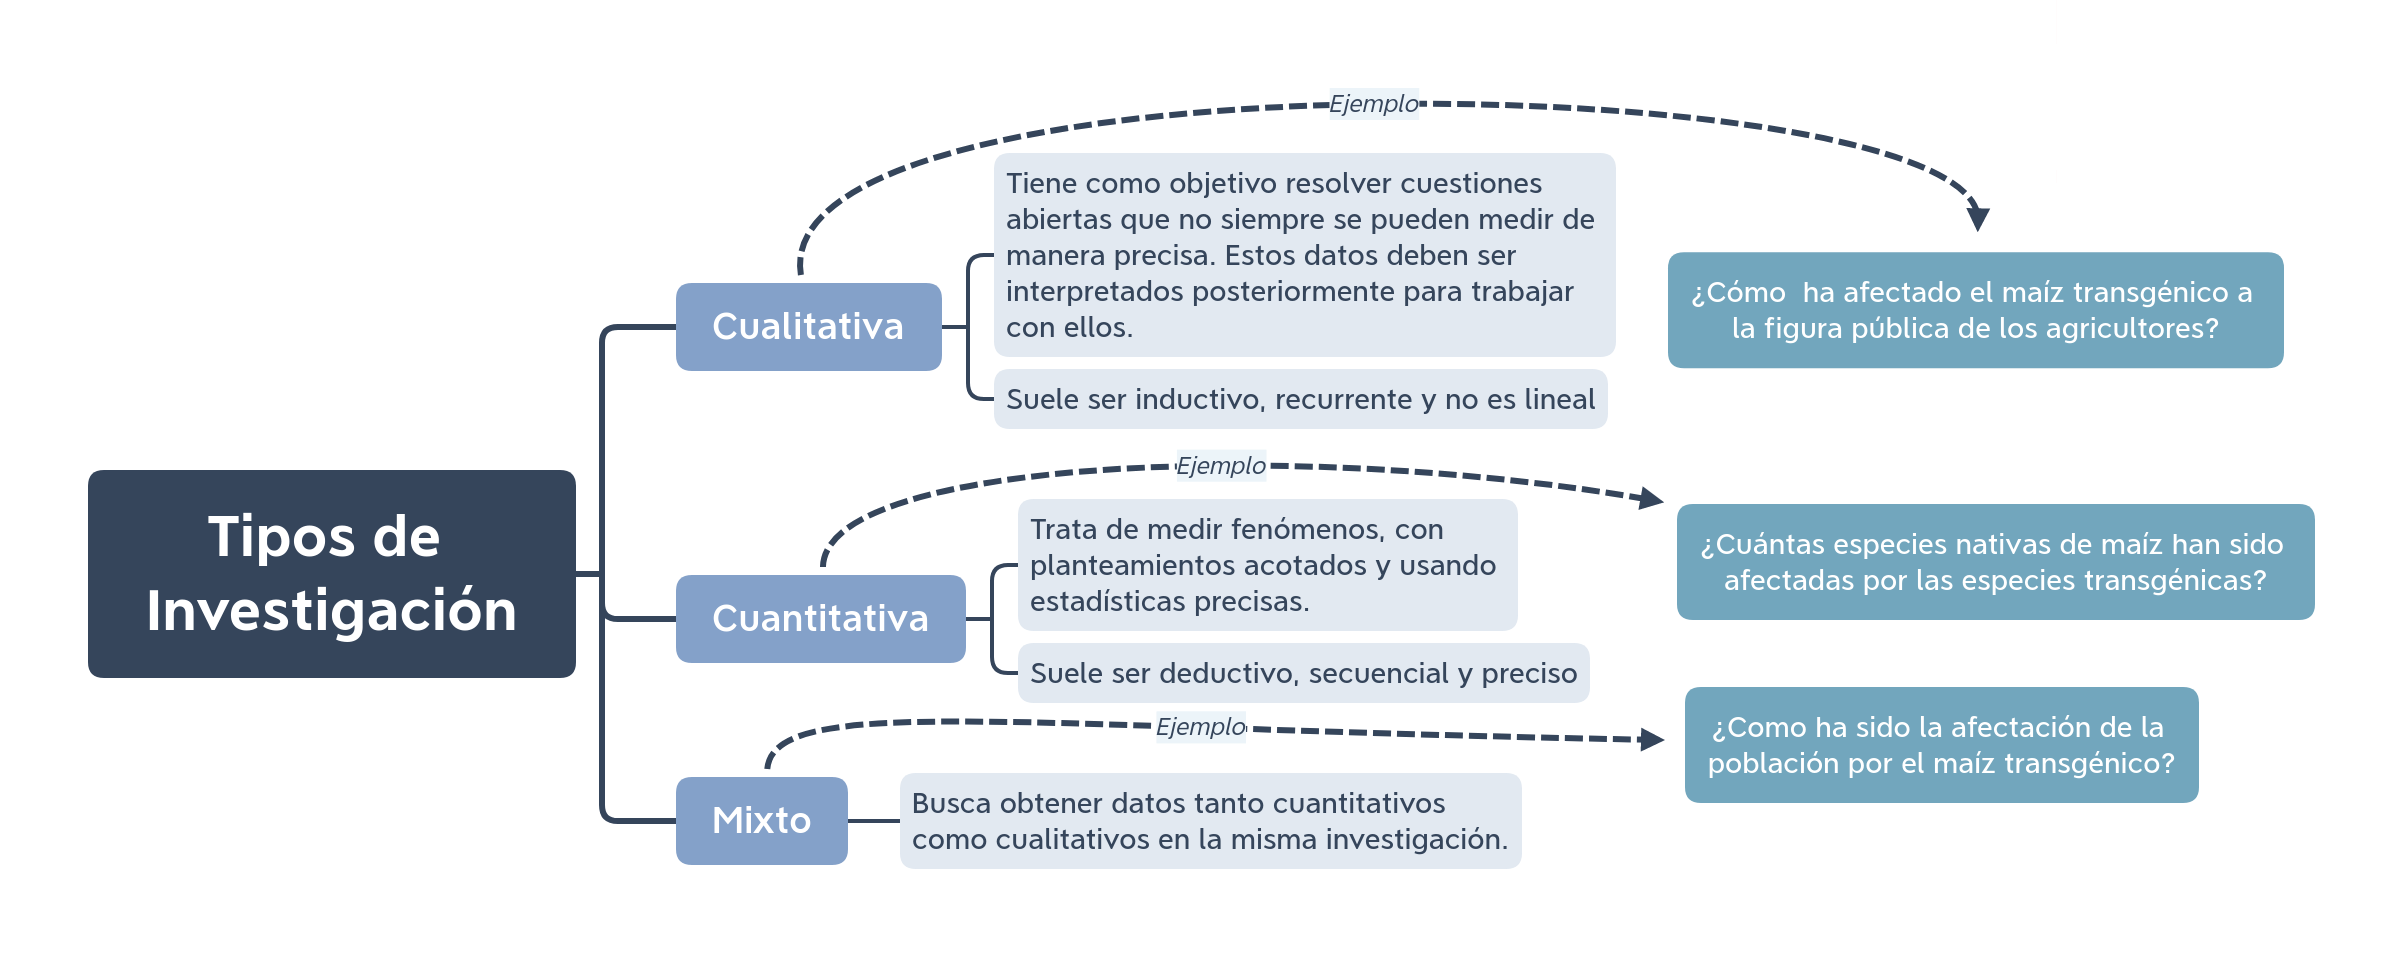
\includegraphics[width=0.79\textwidth, angle=90]{Tipos-Investigacion.png}
		\caption{Tipos de Investigación}
		\label{fig: investigacion}
	\end{figure}


\subsection{Ejemplos}

	\begin{description}
		\item[Cualitativo] El art\'iculo \textit{Diseño de fármacos asistido por computadora}\cite{cadFarmacos} trata de identificar \textbf{cual} es el \textit{estado del arte} en las herramientas de la materia. 
		\item[Cuantitativo] Por otro lado, el art\'iculo \textit{MEDICIÓN DE EMISIONES FUGITIVAS...}\cite{cuantitativos} busca encontrar una \textbf{medici\'on} precisa de algo.
		\item[Mixto] Por \'ultimo el art\'iculo \cite{mixto} trata de estudiar y medir el an\'alisis del m\'etodo descrito.
	\end{description}


\section{Problem\'aticas de Biotecnolog\'ia}

\begin{enumerate}
	\item C\'omo crear plantas fluorescentes
		\begin{description}
			\item [Por qu\'e?] Uno de mis mayores intereses en la ciencia, es la divulgaci\'on de esta, principalmente a nivel de educaci\'on b\'asica que es donde los alumnos son m\'as receptivos y curiosos.
			\item [Tipo] Dado que es necesario crear una t\'ecnica para poder hacer ciertas plantas fluorescentes, esta investigaci\'on deber\'ia de tener un engoque \textbf{cualitativo}
		\end{description}
	
	\item Medici\'on de contaminaci\'on de zonas urbanas
		\begin{description}
			\item [Por qu\'e?] La contaminaci\'on es un tema atacado por un ejercito de areas y carreras. Y la biotecnolog\'ia esta dentro de estas.
			\item [Tipo] Dado que busca medir ciertos parametros, este debe ser un proyecto de investigaci\'on \textit{cuantitativo}.
		\end{description}
		
	\item Identificaci\'on autom\'atica de patrones gen\'omicos en grupos de poblaci\'on.
		\begin{description}
			\item [Por qu\'e?] Los datos gen\'omicos son una enorme mara\~na de datos que a\'un no comprendemos del todo. Las ciencias de la computaci\'on tienen areas experta en buscar patrones que nosotros a\'un no encontramos. La uni\'on de estas tecnolog\'ias podr\'ian apoyar en estas investigaciones.
			\item [Tipo] Creo que esto debe de ser estudiado desde un aspecto \textit{cuantitativo}.
		\end{description}
		
	\item T\'ecnicas de repoblación de ecosistemas víctimas de desastres humanos.
		\begin{description}
			\item [Por qu\'e?] Qu\'e mejor m\'etodo para deshacer nuestro desastre con la naturaleza que la misma naturaleza? El uso de boitecnolog\'ia para volver a poblar ecosistemas permite que esta sea de manera m\'as org\'anica y fiel a un proceso que sea sustentable en el tiempo.
			\item [Tipo] Este proyecto debee tener un enfoque \textbf{cualitativo}, ya que trata de encontrar t\'ecnicas para cumplir con un ovjetivo.
		\end{description}
		
	\item Optimizaci\'on de limpieza de aguas residuales.
		\begin{description}
			\item [Por qu\'e?] El uso de bioreactores y biotecnolog\'ias para el tratamiento del agua parece una de las t\'ecnicas m\'as novedosas y con menor huella ecol\'ogica para esto.
			\item [Tipo] Esta debe ser una investigaci\'on con enfoque \textbf{mixto}, ya que primero se deben entender los m\'etodos actuales, replantearlos en caso de ser necesarios y leugo medir su desempe\~no para ver que tanto se optimiz\'o el proceso.
			
		\end{description}
\end{enumerate}


%%%%%%%%%%%%%%%%%%%%%%%%%%%%%%%%
%%         Bibliografia        %%
%%%%%%%%%%%%%%%%%%%%%%%%%%%%%%%%%%
\newpage
\begin{thebibliography}{X}
	\bibitem[Cadena, 2017]{tipos} Cadena-Iñiguez, P., Rendón-Medel, R., Aguilar-Ávila, J., Salinas-Cruz, E., Cruz-Morales, F.R., \& Sangerman-Jarquín, D.Ma.. (2017). \textit{Métodos cuantitativos, métodos cualitativos o su combinación en la investigación: un acercamiento en las ciencias sociales}. \textbf{Revista mexicana de ciencias agrícolas}, 8(7), 1603-1617. Recuperado en 30 de septiembre de 2020, de \url{http://www.scielo.org.mx/scielo.php?script=sci_arttext&pid=S2007-09342017000701603&lng=es&tlng=es.}

	\bibitem[Prieto, 2019]{cadFarmacos} Prieto-Martínez, F. D., \& Medina-Franco, J. L.. (2018). \textit{Diseño de fármacos asistido por computadora: cuando la informática, la qu\'imica y el arte se encuentran.} TIP. Revista especializada en ciencias qu\'imico-biol\'ogicas, 21(2), e201826. Epub 03 de septiembre de 2020. \url{https://doi.org/10.22201/fesz.23958723e.2018.2.6}
	
	\bibitem[Hernández, 2017]{cuantitativos} Hernández Sánchez, B. R., \& Quezada Aguilera, V. M. (2017). \textit{MEDICIÓN DE EMISIONES FUGITIVAS DE DEPÓSITOS DE JALES EN EL MINERAL DEL CEDRO Y EXPOSICIÓN DE LA POBLACIÓN DE LA COMUNIDAD}. Jóvenes en la Ciencia - Universidad de Guanajuato. \url{http://www.jovenesenlaciencia.ugto.mx/index.php/jovenesenlaciencia/article/view/1792}
	
	\bibitem[Rueda, 2018]{mixto} Rueda Martinez, E. I., \& Castillo Herrera, I. J. (2018). \textit{ELABORACIÓN Y ANÁLISIS DE LOMBRICOMPOSTA PARA SU APROVECHAMIENTO EN ÁREAS ARBOLADAS DE LA ENMSI}. {Jóvenes en la Ciencia - Universidad de Guanajuato}. \url{http://www.jovenesenlaciencia.ugto.mx/index.php/jovenesenlaciencia/article/view/2858}
	
\end{thebibliography}

	

\end{document}